\documentclass[11pt,a4paper]{article}

\usepackage[margin=0.92in]{geometry}
\usepackage[T1]{fontenc}
\usepackage{lmodern}
\usepackage{microtype}
\usepackage{amsmath,amssymb,mathtools}
\usepackage{booktabs}
\usepackage{tabularx}
\usepackage{longtable}
\usepackage{array}
\usepackage{enumitem}
\usepackage{xcolor}
\usepackage{hyperref}
\usepackage{fancyhdr}
\usepackage[most]{tcolorbox}
\usepackage{tikz}
\usetikzlibrary{arrows.meta,positioning,shapes.geometric,shapes.symbols,fit,calc,backgrounds,matrix}

\definecolor{atlasblue}{HTML}{173B57}
\definecolor{atlascyan}{HTML}{2F9CBB}
\definecolor{atlasgold}{HTML}{C9972E}
\definecolor{atlasgreen}{HTML}{3F7D58}
\definecolor{atlasred}{HTML}{B94A48}
\definecolor{atlaspurple}{HTML}{6B5CA5}
\definecolor{atlasink}{HTML}{1F2933}
\definecolor{atlasslate}{HTML}{52616B}
\definecolor{atlaspaper}{HTML}{F7F8F3}
\definecolor{softblue}{HTML}{EAF4F8}
\definecolor{softgold}{HTML}{FFF4D8}
\definecolor{softgreen}{HTML}{EAF6ED}
\definecolor{softred}{HTML}{FBEAEA}
\definecolor{softpurple}{HTML}{F0EDFA}

\hypersetup{
  colorlinks=true,
  linkcolor=atlasblue,
  citecolor=atlasblue,
  urlcolor=atlascyan,
  pdftitle={The Universal Systems Compiler and The Motif Atlas},
  pdfauthor={Nikit Phadke}
}

\setlength{\parindent}{0pt}
\setlength{\parskip}{0.62em}
\setlength{\headheight}{22pt}
\setlist{itemsep=0.25em,topsep=0.35em,leftmargin=*}
\renewcommand{\arraystretch}{1.14}
\emergencystretch=2em

\pagestyle{fancy}
\fancyhf{}
\lhead{\footnotesize\textsc{The Universal Systems Compiler}}
\rhead{\footnotesize\thepage}
\renewcommand{\headrulewidth}{0.35pt}
\renewcommand{\headrule}{\hbox to\headwidth{\color{atlasblue}\leaders\hrule height \headrulewidth\hfill}}

\newcolumntype{Y}{>{\raggedright\arraybackslash}X}
\newcolumntype{L}[1]{>{\raggedright\arraybackslash}p{#1}}

\newcommand{\motif}[1]{\textbf{\textcolor{atlasblue}{#1}}}
\newcommand{\question}[1]{\textit{#1}}
\newcommand{\comp}{\mathbin{\otimes}}
\newcommand{\MotifSpace}{\mathcal{M}^{32}}

\newtcolorbox{thesisbox}{
  enhanced,
  colback=softblue,
  colframe=atlasblue,
  boxrule=0.6pt,
  arc=2.5pt,
  left=9pt,right=9pt,top=7pt,bottom=7pt
}

\newtcolorbox{principlebox}[1]{
  enhanced,
  title=#1,
  colback=softgold,
  colframe=atlasgold!85!black,
  coltitle=atlasink,
  fonttitle=\bfseries,
  boxrule=0.6pt,
  arc=2.5pt,
  left=9pt,right=9pt,top=7pt,bottom=7pt
}

\newtcolorbox{diagnosticbox}[1]{
  enhanced,
  title=#1,
  colback=softred,
  colframe=atlasred,
  coltitle=atlasink,
  fonttitle=\bfseries,
  boxrule=0.6pt,
  arc=2.5pt,
  left=9pt,right=9pt,top=7pt,bottom=7pt
}

\newtcolorbox{definitionbox}[1]{
  enhanced,
  title=#1,
  colback=softgreen,
  colframe=atlasgreen!80!black,
  coltitle=atlasink,
  fonttitle=\bfseries,
  boxrule=0.6pt,
  arc=2.5pt,
  left=9pt,right=9pt,top=7pt,bottom=7pt
}

\newtcolorbox{compilerbox}[1]{
  enhanced,
  title=#1,
  colback=softpurple,
  colframe=atlaspurple,
  coltitle=atlasink,
  fonttitle=\bfseries,
  boxrule=0.6pt,
  arc=2.5pt,
  left=9pt,right=9pt,top=7pt,bottom=7pt
}

\tikzset{
  motifnode/.style={rounded corners=2pt, draw=atlasblue, fill=softblue, line width=0.55pt, align=center, font=\scriptsize, inner sep=4pt},
  hubnode/.style={rounded corners=2pt, draw=atlasgold!90!black, fill=softgold, line width=0.8pt, align=center, font=\scriptsize\bfseries, inner sep=4pt},
  process/.style={rounded corners=3pt, draw=atlasblue, fill=softblue, line width=0.65pt, align=center, font=\small, minimum width=2.5cm, minimum height=0.85cm},
  layer/.style={rounded corners=3pt, draw=atlaspurple, fill=softpurple, line width=0.65pt, align=center, font=\small, minimum width=3.0cm, minimum height=0.88cm},
  edge/.style={-{Latex[length=2.3mm]}, line width=0.55pt, draw=atlasslate},
  strongedge/.style={-{Latex[length=2.6mm]}, line width=0.8pt, draw=atlasblue},
  dashededge/.style={-{Latex[length=2.2mm]}, dashed, line width=0.55pt, draw=atlasslate}
}

\title{\vspace{-2.2em}\Huge\textbf{The Universal Systems Compiler\\[-0.05em]\Large and The Motif Atlas}\\[0.55em]
\large A Structural Alphabet, Grammar, Geometry, and Compiler for Cross-Domain Transfer}
\author{\Large Nikit Phadke}
\date{June 2026}

\begin{document}
\maketitle
\thispagestyle{empty}

\begin{center}
\begin{tikzpicture}[node distance=1.2cm, scale=0.84, transform shape]
  \node[process, fill=softgreen, draw=atlasgreen!80!black] (domain) {Domain-specific\\system description};
  \node[process, right=of domain] (lexer) {Lexer\\motif tokens};
  \node[process, right=of lexer] (ast) {Parser\\motif AST};
  \node[process, right=of ast] (semantic) {Semantic\\analysis};
  \node[process, right=of semantic, fill=softgold, draw=atlasgold!80!black] (output) {Patterns, diagnostics,\\and code generation};
  \draw[strongedge] (domain) -- (lexer);
  \draw[strongedge] (lexer) -- (ast);
  \draw[strongedge] (ast) -- (semantic);
  \draw[strongedge] (semantic) -- (output);
\end{tikzpicture}
\end{center}

\begin{abstract}
This paper introduces the Universal Systems Compiler: a framework for translating any system from any domain into a shared structural intermediate representation. Its alphabet is the Motif Atlas: thirty-two substrate-independent structural concerns that recur across computing, biology, economics, organizations, psychology, and civilizations. Its grammar is the composition graph. Its physics is grounded in the Free Energy Principle. Its geometry is a thirty-two-dimensional motif coordinate space. Its machine is a compiler pipeline that lexes domain language into motifs, parses Boundary-nested ASTs, validates composition and valence, detects structural collisions, diagnoses missing or impoverished motifs, and generates domain-specific interventions. The central claim is that hard problems are rarely domain-specific: they are sparse regions of motif space, and solutions can be found in domains where the same structural region is dense.
\end{abstract}

\begin{thesisbox}
\textbf{Core thesis.} Human knowledge is organized by substrate, but many of its deepest solutions are structural. The Motif Atlas makes those structures visible, searchable, and transferable.
\end{thesisbox}

\tableofcontents
\newpage

\section{The Problem}

A database engineer ensuring cache consistency, a molecular biologist studying chromosome alignment during mitosis, and a diplomat mediating a border dispute are solving the exact same structural problem: how do copies that have diverged arrive at a consistent state under constraints?

Historically, these domains could not share solutions because they lacked a shared language. The database engineer speaks of CRDTs and eventual consistency. The biologist speaks of checkpoint kinases and spindle assembly. The diplomat speaks of confidence-building measures and territorial integrity. Three vocabularies. One structural problem. Zero transfer.

This is not an isolated case. Markets discovering prices, immune systems identifying pathogens, and search engines ranking pages all solve the same structural problem: how does distributed \motif{Feedback} under \motif{Scarcity} converge on accurate \motif{Representation}? Legislatures passing laws, cell nuclei regulating gene expression, and operating systems managing permissions all solve: how does \motif{Authority} enforce \motif{Invariants} across \motif{Hierarchical} scopes?

The structural problems are universal. The solutions are locked inside domains. Human knowledge is organized by substrate --- physics in one building, biology in another, economics in a third, governance in a fourth --- when the structural knowledge in these buildings is largely the same knowledge expressed in different vocabularies.

The Universal Systems Compiler solves this by introducing a shared structural alphabet --- the Motif Atlas --- and a compilation pipeline that transforms any system from any domain into a common intermediate representation where structural solutions become visible, searchable, and transferable.

\begin{figure}[ht]
\centering
\begin{tikzpicture}[node distance=0.85cm and 1.0cm]
  \node[motifnode, fill=softgreen, draw=atlasgreen!80!black] (db) {Database\\engineer};
  \node[motifnode, below=of db, fill=softgreen, draw=atlasgreen!80!black] (bio) {Molecular\\biologist};
  \node[motifnode, below=of bio, fill=softgreen, draw=atlasgreen!80!black] (dip) {Diplomat};
  \node[hubnode, right=2.0cm of bio, minimum width=4.1cm] (problem) {Copies diverge;\\consistency must be restored\\under constraints};
  \node[motifnode, right=2.0cm of problem] (sol) {Shared motifs:\\Replication, Synchronization,\\Reconciliation, Invariant, Authority};
  \draw[edge] (db) -- (problem);
  \draw[edge] (bio) -- (problem);
  \draw[edge] (dip) -- (problem);
  \draw[strongedge] (problem) -- (sol);
\end{tikzpicture}
\caption{Different substrates, one structural problem. The compiler removes domain vocabulary and exposes the common motif signature.}
\end{figure}

\section{The Motif}

\begin{definitionbox}{Definition: motif}
A motif is a recurring structural concern that arises in complex systems independently of what those systems are made of. Each motif is identified by a fundamental question that recurs across computing, biology, economics, organizations, psychology, and civilizations. The question is universal. The answers are domain-specific.
\end{definitionbox}

This distinction between the question and the answer is foundational. The Observer pattern, the Pub-Sub pattern, and the Event Bus pattern are three different answers in three different contexts. They are all responses to the same question: how does the outcome of a transition influence future transitions? That question is the \motif{Feedback} motif. Design patterns are domain-specific solutions. Motifs are substrate-independent questions that generate those solutions.

A motif earns its place by passing five empirical tests. Recognition: experts across four or more domains recognize it immediately. Transfer: understanding it in one domain demonstrably helps reason about another. Compression: naming it collapses many previously separate phenomena into a single concept. Predictive: its absence in a system predicts specific, observable failure modes. Design: asking ``have we addressed this?'' during design reliably reveals missing components.

\begin{table}[ht]
\centering
\caption{The five empirical tests for admitting a motif into the Atlas.}
\begin{tabularx}{\linewidth}{@{}L{0.18\linewidth}Y@{}}
\toprule
\textbf{Test} & \textbf{Criterion} \\
\midrule
Recognition & Experts across four or more domains recognize it immediately. \\
Transfer & Understanding it in one domain demonstrably helps reason about another. \\
Compression & Naming it collapses many previously separate phenomena into a single concept. \\
Predictive & Its absence in a system predicts specific, observable failure modes. \\
Design & Asking ``have we addressed this?'' during design reliably reveals missing components. \\
\bottomrule
\end{tabularx}
\end{table}

Within the compiler architecture, each motif performs quadruple duty. It is a discrete syntax token for the lexer --- a recognizable symbol in the structural alphabet. It is a floating-point dimension in the vector space --- enabling similarity search across millions of systems. It is a typed graph node in the pattern library --- defining what structural inputs it requires and what capabilities it provides. And it is a diagnostic rule for the semantic analyzer --- enabling the compiler to flag specific structural errors when the motif is missing or malformed.

\begin{figure}[ht]
\centering
\begin{tikzpicture}[node distance=1.1cm]
  \node[hubnode, minimum width=2.4cm, minimum height=1.0cm] (m) {Motif};
  \node[motifnode, above left=of m, minimum width=3.0cm] (token) {Lexer token};
  \node[motifnode, above right=of m, minimum width=3.0cm] (vector) {Vector dimension};
  \node[motifnode, below left=of m, minimum width=3.0cm] (pattern) {Typed graph node};
  \node[motifnode, below right=of m, minimum width=3.0cm] (diagnostic) {Diagnostic rule};
  \draw[edge] (m) -- (token);
  \draw[edge] (m) -- (vector);
  \draw[edge] (m) -- (pattern);
  \draw[edge] (m) -- (diagnostic);
\end{tikzpicture}
\caption{Each motif serves simultaneously as syntax, geometry, pattern type, and diagnostic rule.}
\end{figure}

\section{The Atlas: Thirty-Two Motifs}

\subsection*{Atlas at a Glance}
\addcontentsline{toc}{subsection}{Atlas at a Glance}

\begin{table}[p]
\centering
\caption{The thirty-two motifs as a compact question atlas. Group structure is developed in the sections that follow.}
\scriptsize
\setlength{\tabcolsep}{3pt}
\begin{tabularx}{\linewidth}{@{}L{0.035\linewidth}L{0.15\linewidth}Y@{\hspace{0.8em}}L{0.035\linewidth}L{0.15\linewidth}Y@{}}
\toprule
\textbf{No.} & \textbf{Motif} & \textbf{Question} & \textbf{No.} & \textbf{Motif} & \textbf{Question} \\
\midrule
1 & State & What currently exists? & 17 & Compression & How can less describe more? \\
2 & Transition & How does it change? & 18 & Optimization & What should improve? \\
3 & Invariant & What must remain true after every change? & 19 & Explore/Exploit & Learn or use? \\
4 & Identity & What makes each thing uniquely itself? & 20 & Self-Reference & When does a system reference itself? \\
5 & Boundary & What separates inside from outside? & 21 & Composition & How do pieces combine? \\
6 & Terminal State & When is it done? & 22 & Hierarchy & How do small things form larger things under direction? \\
7 & Decay & What degrades without maintenance? & 23 & Modularity & What can change independently? \\
8 & Storage & Where does information persist? & 24 & Abstraction & What can be hidden? \\
9 & Addressing & How do you find what you need? & 25 & Emergence & How do micro-behaviors produce macro-properties? \\
10 & Replication & Can multiple copies exist? & 26 & Scarcity & What is limited? \\
11 & Synchronization & How do copies stay consistent? & 27 & Queue & Who waits? \\
12 & Representation & How is reality encoded? & 28 & Scheduling & Who gets resources next? \\
13 & Feedback & How does the outcome of a transition influence future transitions? & 29 & Communication & How does information move? \\
14 & Prediction & What happens next? & 30 & Authority & Who decides? \\
15 & Search & How do you find a valid path? & 31 & Reconciliation & How do divergent states converge? \\
16 & Model & What internal simulation exists? & 32 & Negotiation & How do agents with competing interests reach agreement? \\
\bottomrule
\end{tabularx}
\end{table}

\subsection{Group A: Existence and Change}

\subsubsection{1. State --- \question{What currently exists?}}

A snapshot of system configuration at a moment in time. The most fundamental motif --- every other motif either reads, writes, or constrains state. Without state, there is nothing to change, protect, communicate, or reason about.

When state is absent or implicit, system behavior becomes unpredictable. You cannot debug what you cannot inspect. You cannot reproduce what you cannot capture. You cannot verify what you cannot observe.

State manifests as CPU registers, database rows, and Petri net markings in computing. As cellular chemistry, phenotype, and ion channel configurations in biology. As balance sheets, price vectors, and inventory levels in economics. As headcount, org charts, and active policies in organizations. As belief states, mood, and working memory contents in psychology. As legal codes, territorial control, and cultural norms in civilization.

\subsubsection{2. Transition --- \question{How does it change?}}

A rule mapping one state to another. The atomic unit of change. Without transitions, state is inert --- nothing happens, nothing evolves, nothing computes. The system is frozen in its initial configuration.

Transition manifests as CPU instructions and Petri net firings in computing. As chemical reactions, action potentials, and gene expression switches in biology. As transactions, trade executions, and monetary transfers in economics. As policy actions, hiring decisions, and process steps in organizations. As learning events, attitude shifts, and decisions in psychology. As legislation, revolution, and treaty ratification in civilization.

\subsubsection{3. Invariant --- \question{What must remain true after every change?}}

A constraint that must hold before and after every transition. Invariants define the boundary between legal and illegal state changes. They are what make systems governable. Without invariants, transitions are unconstrained, optimization produces gaming, and the system's essential character --- its soul --- is undefined.

This is not metaphor. An optimizer without invariants will find every loophole, every exploit, every unintended path to its objective. This is true whether the optimizer is a reinforcement learning agent, a market participant, a politician, or an evolving organism. Invariant absence predicts gaming and exploitation as structural inevitabilities.

Invariant manifests as type safety, referential integrity, and ACID properties in computing. As conservation laws, homeostasis, and enzyme specificity in biology. As the accounting equation, no-arbitrage conditions, and contract law in economics. As bylaws, compliance requirements, and SLAs in organizations. As cognitive consistency, moral axioms, and identity coherence in psychology. As constitutional provisions, human rights, and treaty obligations in civilization.

\subsubsection{4. Identity --- \question{What makes each thing uniquely itself?}}

A stable reference that persists across state changes. Identity is what allows you to say ``this is the same entity'' after a transition has occurred. Two database rows can have identical content but different identities. A person can change every belief, every cell, every habit, and remain the same person. Identity is about reference, not content.

When identity is absent, duplicates accumulate, entities merge incorrectly, and the system cannot distinguish ``same content'' from ``same entity'' from ``same entity over time.'' Entire classes of errors arise from confusing value equality with reference identity.

Identity manifests as memory addresses, PIDs, UUIDs, and primary keys in computing. As DNA sequences, cell lineage markers, and fingerprints in biology. As Tax IDs, ISINs, account numbers, and LEIs in economics. As employee IDs, entity registrations, and brands in organizations. As self-concept, proper names, and autobiographical continuity in psychology. As national identity, cultural markers, and ethnic identity in civilization.

\subsubsection{5. Boundary --- \question{What separates inside from outside?}}

A partition of the universe into system and environment. Boundary is the precondition for agency --- without it, there is no ``inside'' to have state and no ``outside'' to communicate with. Every system that exists has decided what is inside it and what is not.

Within the compiler architecture, Boundary holds a special status: it is the scope delimiter of reality. Just as curly braces create scopes in a programming language, Boundaries create scopes in the motif AST. Every Boundary that contains other structure opens a new level in the hierarchy. Boundary is the parenthesis of reality. Without it, there is only a primordial soup of State and Transition colliding without structure. The moment a lipid bilayer forms in the ocean, or a firewall segments a network, or humans draw a line in the dirt and call it a city --- the first parenthesis opens. A scope is defined. Local state can be protected. An Abstract Syntax Tree can be parsed. Structure begins.

When boundary is absent, there is no isolation, no protection, no modularity. Everything leaks into everything. Security is impossible. The system cannot define itself.

Boundary manifests as firewalls, process isolation, containers, and API surfaces in computing. As cell membranes, blood-brain barriers, and nuclear envelopes in biology. As legal entity boundaries and regulatory perimeters in economics. As department walls, security clearances, and NDA scopes in organizations. As ego boundaries, personal space, and psychological defenses in psychology. As national borders, sovereignty, and territorial waters in civilization.

\begin{principlebox}{Boundary as the parenthesis of reality}
Every scope-defining Boundary opens a level in the motif AST. Local state, local invariants, local authority, and local communication only become parseable after a Boundary defines inside and outside.
\end{principlebox}

\subsubsection{6. Terminal State --- \question{When is it done?}}

A state from which no further transitions are needed or possible. Terminal states turn open-ended processes into bounded ones. Without them, systems run forever --- or until they exhaust resources. There is no definition of done.

Terminal State manifests as HALT states, acceptance states, and fixpoints in computing. As apoptosis, terminal differentiation, and death in biology. As loan settlement, contract fulfillment, and bankruptcy discharge in economics. As project completion, case closure, and retirement in organizations. As goal satisfaction and grief resolution in psychology. As treaty signing, independence, and constitutional ratification in civilization.

\subsubsection{7. Decay --- \question{What degrades without maintenance?}}

The tendency of systems toward disorder in the absence of directed effort. Decay is the only negative motif --- it describes not a capability but an inevitability. It is what happens when other motifs stop operating. Decay is what makes all other motifs necessary: without it, you could build a system once and walk away. With it, every system requires continuous investment in maintenance, repair, and renewal.

Decay is the most underrecognized motif across all domains. Its underrecognition is itself a source of systemic failure --- systems that do not account for their own degradation accumulate invisible structural debt until catastrophic failure.

Decay manifests as bit rot, software decay, clock drift, and data corruption in computing. As aging, mutation accumulation, and protein misfolding in biology. As depreciation, inflation, and market entropy in economics. As bureaucratic drift, culture erosion, and knowledge attrition in organizations. As memory decay, skill atrophy, and habit erosion in psychology. As institutional rot, language drift, and civilizational decline in civilization.

\subsection{Group B: Memory and Persistence}

\subsubsection{8. Storage --- \question{Where does information persist?}}

A bounded region where state survives across time. Storage converts ephemeral information into durable knowledge. Without storage, every transition starts from scratch --- there is no memory, no accumulation, no learning. The system has no history.

Storage manifests as RAM, disk, databases, and register files in computing. As DNA, epigenome, synaptic weights, and bone structure in biology. As ledgers, vaults, warehouses, and reserves in economics. As filing cabinets, wikis, institutional memory, and archive policies in organizations. As long-term memory, procedural memory, and cultural memory in psychology. As libraries, archives, oral traditions, and monuments in civilization.

\subsubsection{9. Addressing --- \question{How do you find what you need?}}

A systematic way to locate a specific entity. Addressing turns the abstract concept of identity into a practical retrieval operation. Without it, stored information is inaccessible --- a library without a catalog. Knowledge exists but cannot be found.

Addressing manifests as URLs, memory addresses, file paths, and DNS in computing. As gene loci, receptor binding sites, and neural coordinates in biology. As account numbers, SWIFT codes, and ticker symbols in economics. As job titles, email addresses, and desk numbers in organizations. As proper names, mental indices, and pronouns in psychology. As GPS coordinates, postal addresses, and country codes in civilization.

\subsubsection{10. Replication --- \question{Can multiple copies exist?}}

Creating copies of stored information across locations. Replication introduces a fundamental tradeoff: it buys availability and resilience at the cost of consistency risk. Once copies exist independently, they can diverge --- creating the structural need for Synchronization and Reconciliation.

Replication manifests as caches, CDNs, database replicas, and RAID in computing. As cell division, viral replication, and horizontal gene transfer in biology. As franchises, subsidiaries, and branch offices in economics. As SOP templates, training programs, and branch replication in organizations. As meme propagation, cultural transmission, and imitation in psychology. As cultural diffusion, diaspora, and colonial replication in civilization.

\subsubsection{11. Synchronization --- \question{How do copies stay consistent?}}

Ensuring that replicated copies converge to a consistent state. This requires detecting divergence (Feedback), defining what consistent means (Invariant), and the authority to enforce convergence. Synchronization is the defining problem of distributed systems, multicellular organisms, and multi-branch organizations alike.

When synchronization is absent, copies diverge silently. Different parts of the system believe different things. Conflicts go undetected. Corruption spreads.

Synchronization manifests as cache coherence protocols, Paxos, Raft, and CRDTs in computing. As chromosome alignment during mitosis and circadian synchronization in biology. As auditing, clearinghouse reconciliation, and mark-to-market in economics. As standup meetings, status reports, and cross-team syncs in organizations. As social norming and consensus formation in psychology. As treaty compliance, international standards, and UTC in civilization.

\subsection{Group C: Intelligence and Learning}

\subsubsection{12. Representation --- \question{How is reality encoded?}}

A mapping from external reality to internal state. Without representation, a system cannot reason about anything beyond its immediate sensory inputs. The quality of a system's representations determines the ceiling on its intelligence. A system cannot reason beyond what its representations can express.

Representation manifests as binary encoding, data structures, embeddings, and knowledge graphs in computing. As DNA codons, neural firing patterns, and receptor configurations in biology. As double-entry bookkeeping, price-as-information, and financial models in economics. As org charts, process maps, KPI dashboards, and strategic plans in organizations. As mental models, schemas, categories, and prototypes in psychology. As written law, maps, language, calendars, and historical records in civilization.

\subsubsection{13. Feedback --- \question{How does the outcome of a transition influence future transitions?}}

The routing of output information back as input. Feedback is what converts a static system into a learning system. Without it, errors persist indefinitely and adaptation is impossible. Negative feedback stabilizes; positive feedback amplifies. Both are instances of the same structural concern: the loop.

A critical principle: a motif can be present but architecturally impoverished. Feedback is the clearest example. Every domain has Feedback, but the architectural richness varies enormously. Biology's Feedback has population redundancy --- millions of organisms providing a robust signal from individually noisy outcomes. Markets' Feedback has self-correcting aggregation --- bad prices create arbitrage opportunities that destroy them. Science's Feedback has validation pipelines --- peer review, replication, statistical standards. Governance's Feedback has constitutional constraints --- the loop cannot produce certain outcomes. A system with Feedback as a bare scalar from a single source with no validation, no aggregation, no constraints, and no redundancy has the weakest Feedback architecture in any domain --- and this architectural poverty is often the root cause of every problem the field is trying to solve.

Feedback manifests as error signals, test results, and monitoring alerts in computing. As natural selection, immune response, and pain/pleasure in biology. As profit/loss, market correction, and customer complaints in economics. As performance reviews, retrospectives, and audit findings in organizations. As emotion, proprioception, and regret in psychology. As elections, protests, and revolution in civilization.

\subsubsection{14. Prediction --- \question{What happens next?}}

An internal model generating expected future states. Prediction separates reactive systems from proactive ones. It arises when representations are iteratively refined by feedback to the point where they anticipate rather than merely record.

When prediction is absent, the system is purely reactive --- always behind, always surprised.

Prediction manifests as branch prediction, prefetch, and LLM next-token generation in computing. As immune memory, classical conditioning, and anticipatory behavior in biology. As futures markets, analyst forecasts, and yield curves in economics. As strategic planning, demand forecasting, and risk assessment in organizations. As anticipation, expectation, and theory of mind in psychology. As intelligence agencies and actuarial science in civilization.

\textbf{Composition:} Representation (12) $\comp$ Feedback (13).

\subsubsection{15. Search --- \question{How do you find a valid path?}}

Systematic exploration of a possibility space to find a configuration satisfying constraints. Search is what a system does when it does not already know the answer --- it enumerates candidates and tests them. The strategy of exploration is what distinguishes intelligent search from brute force.

Search manifests as A*, SAT solvers, and binary search in computing. As evolutionary search, immune repertoire generation, and foraging in biology. As market discovery, price discovery, and venture capital in economics. As R\&D pipelines, hiring funnels, and strategic options analysis in organizations. As problem-solving, brainstorming, and mental simulation in psychology. As geographic exploration, the scientific method, and legal discovery in civilization.

\subsubsection{16. Model --- \question{What internal simulation exists?}}

A bounded internal simulation of external reality. Models enable counterfactual reasoning --- ``what would happen if?'' This is qualitatively different from representation (which encodes what IS) and prediction (which anticipates what WILL BE). A model simulates what COULD BE.

When model is absent, the system cannot reason counterfactually. It cannot plan ahead or evaluate hypotheticals.

\textbf{Composition:} Representation (12) $\comp$ Prediction (14) $\comp$ Boundary (5).

\subsubsection{17. Compression --- \question{How can less describe more?}}

Encoding maximum information in minimum space. This is not merely a technical operation. Compression is understanding. A scientific theory is a compression of observed phenomena. A proverb is a compression of lived experience. A constitution is a compression of governance principles. The ability to compress is the ability to find the structure beneath the surface.

When compression is absent, the system drowns in data without understanding. Storage and compute grow without bound. No generalization occurs.

\textbf{Composition:} Representation (12) $\comp$ Scarcity (26).

\subsubsection{18. Optimization --- \question{What should improve?}}

Directed improvement under constraints. Optimization arises when prediction, search, and scarcity combine to produce systematic pursuit of better states. It is what gives purpose to feedback loops.

\textbf{Composition:} Prediction (14) $\comp$ Search (15) $\comp$ Scarcity (26).

\subsubsection{19. Explore/Exploit --- \question{Learn or use?}}

The fundamental tradeoff between acquiring new information and acting on existing knowledge. Every intelligent system must balance exploration (trying new things, risking failure) against exploitation (using what works, ensuring returns). Too much exploration wastes resources. Too much exploitation leads to local optima and brittleness.

\subsubsection{20. Self-Reference --- \question{When does a system reference itself?}}

A system that contains, operates on, or is defined in terms of a representation of itself. Self-Reference is the motif that separates systems that can improve themselves from those that cannot. It creates both the most powerful system capabilities --- self-improvement, reflection, meta-reasoning --- and the most dangerous failure modes --- infinite regress, paradox, G\"odelian incompleteness, the halting problem. Power and limitation from the same source.

Self-Reference manifests as self-compiling compilers, quines, and reflection APIs in computing. As autopoiesis, self-replicating RNA, and recursive gene regulation in biology. As derivatives of derivatives and meta-markets in economics. As self-governing organizations in governance. As metacognition and self-awareness in psychology. As constitutional self-amendment and self-determining peoples in civilization.

\subsection{Group D: Structure and Scale}

\subsubsection{21. Composition --- \question{How do pieces combine?}}

Constructing complex wholes from simpler elements. The foundation of all structure. Without composition, there is a flat universe of isolated atoms with no organization. The combination rules matter as much as the parts.

\subsubsection{22. Hierarchy --- \question{How do small things form larger things under direction?}}

Composition with authority --- higher levels coordinate and constrain lower levels. Hierarchy is how complex systems achieve coordination without requiring every element to communicate with every other. It trades local autonomy for global coherence.

\textbf{Composition:} Composition (21) $\comp$ Authority (30).

\subsubsection{23. Modularity --- \question{What can change independently?}}

Bounded parts with well-defined interfaces. What makes complex systems maintainable --- you can change one part without breaking the others. The cost is the overhead of maintaining interfaces.

When modularity is absent, changes cascade unpredictably. Everything is coupled. One change breaks everything.

\textbf{Composition:} Boundary (5) $\comp$ Composition (21).

\subsubsection{24. Abstraction --- \question{What can be hidden?}}

Hiding internal complexity behind a simpler interface. Every successful abstraction is a bet that the hidden details do not matter for the current purpose --- and that bet can be wrong. Every abstraction leaks under sufficient stress. Premature abstraction is debt.

\textbf{Composition:} Boundary (5) $\comp$ Representation (12).

\subsubsection{25. Emergence --- \question{How do micro-behaviors produce macro-properties?}}

Properties that exist at the macro level but not at the component level. Emergence is what makes reductionism insufficient --- knowing everything about individual neurons does not predict consciousness, knowing everything about individual traders does not predict market crashes. The whole is genuinely more than the sum.

\textbf{Composition:} Composition (21) $\comp$ Feedback (13).

\subsection{Group E: Resources and Allocation}

\subsubsection{26. Scarcity --- \question{What is limited?}}

The condition that demand exceeds supply. Scarcity forces choice, and choice is what makes optimization, scheduling, negotiation, and competition necessary. A system with infinite resources does not need to be intelligent. Scarcity is what makes intelligence necessary.

\subsubsection{27. Queue --- \question{Who waits?}}

An ordered collection of pending demands. Queues arise wherever scarce resources must serve multiple requests. They make the hidden cost of scarcity visible: the queue length is the measure of unmet demand.

\textbf{Composition:} Scarcity (26) $\comp$ Composition (21).

\subsubsection{28. Scheduling --- \question{Who gets resources next?}}

A decision procedure for allocating scarce resources across competing demands over time. The scheduling policy encodes the system's values --- fairness, efficiency, urgency, priority. Different policies produce radically different outcomes from the same inputs.

\textbf{Composition:} Queue (27) $\comp$ Authority (30).

\subsection{Group F: Coordination and Governance}

\subsubsection{29. Communication --- \question{How does information move?}}

The transfer of information across a boundary. Communication is the only mechanism by which separate systems can coordinate. Its bandwidth, latency, fidelity, and cost determine the upper bound on coordination quality achievable.

\subsubsection{30. Authority --- \question{Who decides?}}

The asymmetric right to change state or enforce invariants. Authority resolves the fundamental coordination question: when multiple agents disagree about the next transition, whose choice prevails? Without authority, disagreements have no resolution mechanism other than force.

\subsubsection{31. Reconciliation --- \question{How do divergent states converge?}}

The process of detecting divergence between states that should agree, and resolving it under constraints. Reconciliation is where most real-world coordination complexity concentrates. It requires communication (to compare), invariant definition (to know what consistent means), and authority (to resolve what cannot be automatically merged).

When reconciliation is absent, contradictions accumulate. Different parts of the system believe different things. No conflict resolution exists. Divergence grows until the system breaks.

\textbf{Composition:} Communication (29) $\comp$ Invariant (3) $\comp$ Authority (30).

\subsubsection{32. Negotiation --- \question{How do agents with competing interests reach agreement?}}

The process by which agents under scarcity communicate to reach a mutually acceptable outcome. Negotiation is the civilized alternative to unilateral action. Its failure mode is conflict.

\textbf{Composition:} Communication (29) $\comp$ Scarcity (26) $\comp$ Authority (30).

\section{The Grammar: Composition, Valence, and Collisions}

\subsection{The Composition Graph}

Motifs are not independent atoms. They combine according to structural dependencies that form a directed acyclic graph --- the composition grammar of the atlas. Prediction requires Representation and Feedback. Optimization requires Prediction, Search, and Scarcity. Reconciliation requires Communication, Invariant, and Authority.

These dependencies are not arbitrary classifications. They are structural necessities. You cannot anticipate the future (Prediction) without an internal encoding of reality (Representation) refined by past outcomes (Feedback). You cannot improve (Optimization) without anticipation (Prediction), alternatives (Search), and constraints (Scarcity). You cannot resolve divergence (Reconciliation) without information exchange (Communication), a definition of consistency (Invariant), and the power to enforce resolution (Authority).

Six motifs emerge as hubs in the composition graph --- they participate in the most compositions and serve as prerequisites for the largest number of capabilities. These are Representation, Scarcity, Boundary, Authority, Feedback, and Composition. A system missing any hub motif loses access to a large fraction of the composite layer. Hub motifs are structural bottlenecks: adding them unlocks disproportionate capability.

\begin{figure}[ht]
\centering
\begin{tikzpicture}[node distance=0.75cm and 1.0cm]
  \node[hubnode] (rep) {Representation};
  \node[hubnode, below=of rep] (fb) {Feedback};
  \node[motifnode, right=1.25cm of $(rep)!0.5!(fb)$] (pred) {Prediction};
  \node[motifnode, below=of pred] (model) {Model};
  \node[hubnode, below=of fb] (bound) {Boundary};
  \node[motifnode, right=1.3cm of model] (opt) {Optimization};
  \node[motifnode, below=of opt] (recon) {Reconciliation};
  \node[motifnode, above=of opt] (search) {Search};
  \node[hubnode, right=1.35cm of search] (scar) {Scarcity};
  \node[hubnode, right=1.35cm of opt] (auth) {Authority};
  \node[hubnode, right=1.35cm of recon] (comm) {Communication};
  \node[motifnode, below=of auth] (inv) {Invariant};
  \node[hubnode, below=of inv] (compn) {Composition};
  \node[motifnode, right=of compn] (hier) {Hierarchy};
  \node[motifnode, left=of compn] (emerg) {Emergence};
  \draw[edge] (rep) -- (pred);
  \draw[edge] (fb) -- (pred);
  \draw[edge] (rep) -- (model);
  \draw[edge] (pred) -- (model);
  \draw[edge] (bound) -- (model);
  \draw[edge] (pred) -- (opt);
  \draw[edge] (search) -- (opt);
  \draw[edge] (scar) -- (opt);
  \draw[edge] (comm) -- (recon);
  \draw[edge] (auth) -- (recon);
  \draw[edge] (inv) -- (recon);
  \draw[edge] (compn) -- (hier);
  \draw[edge] (auth) -- (hier);
  \draw[edge] (compn) -- (emerg);
  \draw[edge] (fb) |- (emerg);
\end{tikzpicture}
\caption{A simplified composition graph. Hub motifs unlock disproportionate composite capability.}
\end{figure}

\subsection{Emergent Composites}

Systematic exploration of motif pairs --- the Mendeleev method applied to structural knowledge --- reveals composites that pass all five membership tests but were not initially cataloged. These are the predicted elements of the structural periodic table.

Accountability arises from Feedback combined with Authority --- someone must answer for outcomes. Trust arises from Identity combined with Communication --- the ability to verify and rely on the sender. Rule of Law arises from Invariant combined with Authority --- the authorities themselves are bound by rules. Corruption arises from Decay combined with Invariant --- rules stop being enforced as maintenance fails. Runaway arises from Decay combined with Self-Reference --- self-reinforcing degradation that escapes all control, the structural signature shared by cancer, financial bubbles, and bureaucratic ossification.

At higher orders of combination, motif recipes produce recognizable institutions. A market requires five motifs. A democracy requires five. The scientific method requires five. These institutions recur across civilizations because the same motif recipes are the stable solutions to universal structural problems. The atlas is a generative grammar for institutions.

\begin{table}[ht]
\centering
\caption{Examples of emergent composites predicted by motif pairing.}
\begin{tabularx}{\linewidth}{@{}L{0.21\linewidth}L{0.34\linewidth}Y@{}}
\toprule
\textbf{Composite} & \textbf{Motif recipe} & \textbf{Structural meaning} \\
\midrule
Accountability & Feedback $\comp$ Authority & Someone must answer for outcomes. \\
Trust & Identity $\comp$ Communication & The receiver can verify and rely on the sender. \\
Rule of Law & Invariant $\comp$ Authority & Authorities themselves are bound by rules. \\
Corruption & Decay $\comp$ Invariant & Rules stop being enforced as maintenance fails. \\
Runaway & Decay $\comp$ Self-Reference & Self-reinforcing degradation escapes all control. \\
\bottomrule
\end{tabularx}
\end{table}

\subsection{Motif Valence}

Each motif has structural prerequisites --- inputs it requires to function --- and structural provisions --- capabilities it contributes when present. This input-output structure is the motif's valence.

Reconciliation's input valence requires Communication, Authority, and Invariant. Its output valence provides the capability to detect and resolve divergence. If a system claims Reconciliation without sourcing its prerequisites, the claim is structurally invalid --- a dangling valence. The compiler flags this as a composition error.

Valence is what makes cross-domain pattern grafting precise rather than analogical. When a structural pattern is transplanted from one domain to another, the valence requirements must be satisfied at the graft point. A pattern requiring Identity, Boundary, and Authority at its graft point will not successfully instantiate where any of these are missing. The motif types constrain which patterns can be grafted where, eliminating false analogies and ensuring structural compatibility.

\subsection{Motif Collisions}

Some motif combinations are structurally impossible in any substrate. Prediction combined with Self-Reference and Terminal State produces the halting problem --- a system that must predict its own termination, which is provably undecidable. Complete Self-Reference combined with Invariant produces G\"odel's incompleteness --- a system cannot fully prove its own consistency.

These are not engineering limitations. They are structural impossibilities --- motif collisions. The compiler detects them at analysis time, preventing the specification of systems that cannot be built regardless of implementation sophistication.

\begin{diagnosticbox}{Collision registry examples}
\begin{tabularx}{\linewidth}{@{}L{0.42\linewidth}Y@{}}
\toprule
\textbf{Motif collision} & \textbf{Structural impossibility} \\
\midrule
Prediction $\comp$ Self-Reference $\comp$ Terminal State & A system must predict its own termination; the halting problem appears. \\
Complete Self-Reference $\comp$ Invariant & A system attempts to fully prove its own consistency; G\"odelian incompleteness appears. \\
\bottomrule
\end{tabularx}
\end{diagnosticbox}

\section{The Physics: FEP Grounding}

The Free Energy Principle, derived independently by Karl Friston through variational calculus and Bayesian inference, can be derived from motif completeness alone using purely structural arguments.

Three axioms: a system is State bounded by Boundary (it exists as a distinct entity); Decay degrades every bounded system (entropy is universal); every system operates under Scarcity (resources are finite).

From these axioms: a system persisting against Decay must have Transition (it must act to counteract degradation). Under Scarcity, it must have Feedback (it must know whether its actions are working). Feedback refines into Representation. Representation refined by Feedback converges on Prediction. Prediction combined with Representation and Boundary produces Model.

When Prediction diverges from Feedback --- when the world surprises the system --- exactly two responses exist. Update the Representation to match observations (perceptual inference). Or execute Search followed by Transition to change the environment to match the model (active inference). Balancing these under Scarcity is the Explore/Exploit tradeoff.

The correspondence is term-by-term exact. The Markov blanket is the Boundary, with Feedback as sensory states flowing inward and Transition as active states flowing outward. Surprise is prediction error. The generative model is the Model composite. Free energy minimization is persistence against Decay.

Two independent formalisms --- one variational, one structural --- converging on the same architecture constitutes strong evidence that the architecture describes genuine features of reality. The atlas adds beyond the FEP: Self-Reference for self-modeling, Reconciliation for competing hypotheses, Decay combined with Compression for memory consolidation, and Invariant for hard safety constraints that the FEP framework does not address.

\begin{figure}[ht]
\centering
\begin{tikzpicture}[node distance=0.75cm and 0.9cm, scale=0.76, transform shape]
  \node[motifnode] (axiom1) {State bounded\\by Boundary};
  \node[motifnode, below=of axiom1] (axiom2) {Decay};
  \node[motifnode, below=of axiom2] (axiom3) {Scarcity};
  \node[hubnode, right=1.3cm of axiom2] (persist) {Persistence\\pressure};
  \node[motifnode, right=1.25cm of persist] (trans) {Transition};
  \node[hubnode, right=of trans] (feed) {Feedback};
  \node[hubnode, right=of feed] (rep) {Representation};
  \node[motifnode, right=of rep] (pred) {Prediction};
  \node[motifnode, right=of pred] (model) {Model};
  \node[motifnode, below=1.0cm of pred] (surprise) {Prediction error\\/ surprise};
  \node[motifnode, below left=0.85cm and 0.35cm of surprise] (percept) {Update\\Representation};
  \node[motifnode, below right=0.85cm and 0.35cm of surprise] (active) {Search + Transition};
  \draw[edge] (axiom1) -- (persist);
  \draw[edge] (axiom2) -- (persist);
  \draw[edge] (axiom3) -- (persist);
  \draw[strongedge] (persist) -- (trans);
  \draw[strongedge] (trans) -- (feed);
  \draw[strongedge] (feed) -- (rep);
  \draw[strongedge] (rep) -- (pred);
  \draw[strongedge] (pred) -- (model);
  \draw[edge] (model) -- (surprise);
  \draw[edge] (feed) |- (surprise);
  \draw[edge] (surprise) -- (percept);
  \draw[edge] (surprise) -- (active);
\end{tikzpicture}
\caption{A structural derivation of the Free Energy Principle from motif completeness.}
\end{figure}

\section{The Geometry: Coordinate Space Theory}

Every system occupies a point in thirty-two-dimensional motif space. Its coordinates are which motifs it instantiates and how richly. This is not metaphor. It is the operating geometry of structural knowledge.

\textbf{Distance} between systems is structural similarity. Systems close in motif space share structural properties regardless of domain. A cooperative bank and a distributed database --- different vocabulary, different conferences, different literature --- may sit near each other because both instantiate State, Storage, Replication, Invariant, and Authority, and both struggle with Synchronization and Reconciliation. Their proximity is invisible to domain-specific analysis but immediately apparent in the universal coordinates. Solutions transfer between nearby points because structural kinship means shared structural needs.

\textbf{Empty regions} --- positions in motif space populated in some domains but vacant in others --- are undiscovered systems. They are structurally possible but not yet built. The Mendeleev method applied to the full coordinate space identifies these positions and predicts what systems would occupy them. Every empty cell in the original periodic table eventually yielded a new element. Every empty region in motif space is a potential invention.

\textbf{Trajectories} through the space record a field's history. A field that has been adding motifs for decades follows a path through the space. The trajectory's current direction predicts the field's next advance --- the motifs it has not yet added but is approaching.

\textbf{Phase transitions} occur when a system's coordinates cross from zero to nonzero on a hub motif. Adding more Compression to a system that already has some is a smooth improvement. Adding Feedback to a system that has none is a qualitative transformation --- from static to adaptive, from blind to learning. Zero-to-nonzero crossings on hub motifs produce paradigm shifts because hubs unlock large regions of the composite space.

\textbf{The viability manifold} is the subset of motif space where persistent systems can exist. The FEP derivation defines its shape: State, Boundary, Transition, and Feedback at minimum. Systems outside this manifold are structurally unstable --- they either evolve toward it or cease to exist. This is natural selection expressed geometrically.

\textbf{The innovation gradient} at any point in the space points toward the absent motif whose addition would unlock the most composite capabilities. This is computable from the composition graph and it automates the question of where the highest-leverage innovation lies.

\textbf{Universal embeddings.} Motif signatures are structural embeddings. The atlas is a foundation model for systems --- enabling structural similarity search across all domains simultaneously.

\textbf{The core operating principle.} Different domains have explored different regions of motif space to different depths. Dense regions in one domain can be transferred to sparse regions in another via motif coordinates. If a problem is hard in one domain --- if that region of motif space is sparse --- find the domain where it is dense, solve it there, and transfer back. The motif coordinates are the translation layer.

\begin{figure}[ht]
\centering
\begin{tikzpicture}[x=0.92cm,y=0.92cm]
  \draw[->, thick, atlasblue] (0,0) -- (8.3,0) node[right] {Feedback richness};
  \draw[->, thick, atlasblue] (0,0) -- (0,4.6) node[above] {Authority richness};
  \draw[->, thick, atlasblue] (0,0) -- (-2.0,-1.25) node[left] {Boundary richness};
  \fill[softgreen, draw=atlasgreen!80!black, opacity=0.85] (2.0,0.9) ellipse (1.0 and 0.45);
  \node[font=\scriptsize, align=center] at (2.0,0.9) {Software\\distributed systems};
  \fill[softgold, draw=atlasgold!80!black, opacity=0.85] (5.0,2.7) ellipse (1.15 and 0.5);
  \node[font=\scriptsize, align=center] at (5.0,2.7) {Governance\\institutions};
  \fill[softpurple, draw=atlaspurple, opacity=0.85] (3.7,3.7) ellipse (1.05 and 0.45);
  \node[font=\scriptsize, align=center] at (3.7,3.7) {Biological\\systems};
  \fill[softred, draw=atlasred, opacity=0.8] (6.6,1.05) ellipse (0.95 and 0.42);
  \node[font=\scriptsize, align=center] at (6.6,1.05) {Empty\\region};
  \draw[dashededge] (2.8,1.1) .. controls (4.2,1.6) and (5.5,1.3) .. (6.0,1.05);
  \node[font=\scriptsize, align=center, text=atlasred] at (6.6,0.2) {Potential invention};
  \draw[strongedge] (5.2,2.25) -- (6.05,1.35);
  \node[font=\scriptsize, text=atlasblue] at (4.4,1.75) {transfer};
\end{tikzpicture}
\caption{A schematic projection of thirty-two-dimensional motif space. Dense regions in one domain can seed sparse regions in another.}
\end{figure}

\section{The Methodology: Cross-Domain Pipeline}

No hard problem is domain-specific. Every hard problem in domain A has an easier version in some domain B, discoverable through motif signature matching. A problem is hard precisely because the domain has not developed solutions for that region of motif space. Some other domain is dense there.

Different domains are not merely different subjects. They are different optimization engines, each supremely efficient at a different phase of problem-solving.

\textbf{Mathematics} is lean for proof. It establishes what is structurally possible and what is structurally impossible at zero implementation cost. A mathematical proof holds across every substrate simultaneously.

\textbf{Software} is lean for prototyping. A structural hypothesis that would take years to test in biology or governance can be implemented and tested in software in hours. Software is the fastest iteration cycle available.

\textbf{Biology} is lean for optimization. Evolution has explored motif space for three and a half billion years under relentless selection pressure. Its solutions are not merely good --- they are hyper-optimized across timescales no human effort can match.

\textbf{Governance} is lean for hardening. Human institutions have endured millennia of adversarial pressure --- intelligent agents actively trying to exploit, corrupt, and subvert every system. Constitutional design is adversarial robustness engineering.

The pipeline routes each phase to the domain where it is cheapest: \textbf{Prove} the structural properties in mathematics. \textbf{Prototype} the implementation in software. \textbf{Optimize} by studying the biological analogue. \textbf{Harden} by studying the governance analogue. \textbf{Transfer} the combined solution to the target domain through motif coordinates.

Each domain contributes what it is leanest at. The motif space is the common language making contributions composable.

\begin{figure}[ht]
\centering
\begin{tikzpicture}[node distance=0.62cm and 0.7cm, scale=0.88, transform shape]
  \node[layer, fill=softgold, draw=atlasgold!80!black] (math) {Prove\\\footnotesize Mathematics};
  \node[layer, right=of math, fill=softgreen, draw=atlasgreen!80!black] (soft) {Prototype\\\footnotesize Software};
  \node[layer, right=of soft, fill=softpurple, draw=atlaspurple] (bio) {Optimize\\\footnotesize Biology};
  \node[layer, right=of bio, fill=softred, draw=atlasred] (gov) {Harden\\\footnotesize Governance};
  \node[layer, right=of gov, fill=softblue, draw=atlasblue] (target) {Transfer\\\footnotesize Target domain};
  \draw[strongedge] (math) -- (soft);
  \draw[strongedge] (soft) -- (bio);
  \draw[strongedge] (bio) -- (gov);
  \draw[strongedge] (gov) -- (target);
\end{tikzpicture}
\caption{Cross-domain routing: each phase goes to the domain where that phase is cheapest.}
\end{figure}

\section{The Compiler}

\subsection{Architecture}

The compiler separates stochastic creativity from deterministic logic across three layers.

\textbf{Layer 1: The Atlas Kernel.} Pure, deterministic, referentially transparent. Stores the 32 motifs, the composition graph, the collision registry. Runs AST parsing, valence checking, and outputs structural verdicts. This layer embodies the laws of structural physics --- it cannot be negotiated with.

\textbf{Layer 2: The Protocol Engine.} Manages control flow --- when things happen. Maintains the frontier queue, enforces fractal depth limits, dispatches targeted questions to Layer 3, and compiles the final audit record.

\textbf{Layer 3: The Discovery Layer.} The LLM. It reads unstructured text, strips domain metadata, and maps natural language to motif tokens. It assesses fidelity --- whether an implementation is architecturally rich or impoverished. It is the intuition engine, operating under the structural constraints set by Layers 1 and 2.

\begin{figure}[ht]
\centering
\begin{tikzpicture}[node distance=0.55cm]
  \node[layer, minimum width=8.6cm, fill=softpurple, draw=atlaspurple] (l3) {Layer 3: Discovery Layer --- LLM intuition over unstructured text};
  \node[layer, below=of l3, minimum width=8.6cm, fill=softgold, draw=atlasgold!80!black] (l2) {Layer 2: Protocol Engine --- frontier queue, depth limits, audit record};
  \node[layer, below=of l2, minimum width=8.6cm, fill=softblue, draw=atlasblue] (l1) {Layer 1: Atlas Kernel --- motifs, composition graph, collisions, valence};
  \draw[edge] (l3) -- (l2);
  \draw[edge] (l2) -- (l1);
  \draw[dashededge] ([xshift=-3.9cm]l1.north) -- ([xshift=-3.9cm]l3.south);
  \draw[dashededge] ([xshift=3.9cm]l1.north) -- ([xshift=3.9cm]l3.south);
\end{tikzpicture}
\caption{Compiler architecture: stochastic discovery is constrained by deterministic structural physics.}
\end{figure}

\subsection{The Lexer}

The lexer reads domain-specific descriptions and produces a stream of motif tokens. The token vocabulary is the 32 motifs. Domain-specific terms map to universal tokens --- every domain has its own surface language but the tokens are from the same 32-symbol alphabet.

The critical lexer operation is classifying Boundary tokens as scope delimiters. Not every mention of a boundary concept opens a new scope. The lexer must distinguish a Boundary that defines a contained scope from a Boundary referenced as a concept. In formal input languages, this is syntactically explicit. In natural language, the LLM infers scope boundaries from context.

\subsection{The Parser}

The parser takes the motif token stream and builds an Abstract Syntax Tree. The single hierarchical principle is Boundary nesting: every scope-defining Boundary creates a child node; closing a scope returns to the parent. Each node carries a motif signature --- the set of motifs instantiated within that scope.

Three types of edges connect nodes. \textbf{Containment edges} run vertically, representing the parent-child relationship defined by Boundary nesting --- this is the tree structure itself. \textbf{Communication edges} run horizontally between sibling nodes, representing information flow across Boundaries, typed by the motif being communicated. \textbf{Authority edges} run downward from parent to child, representing inherited constraints --- Invariants that bind all descendants. A child can add stricter local Invariants but cannot override inherited ones.

\begin{figure}[ht]
\centering
\begin{tikzpicture}[node distance=0.8cm and 1.2cm]
  \node[hubnode, minimum width=7.4cm, minimum height=0.9cm] (root) {Boundary scope: system};
  \node[motifnode, below left=of root, minimum width=2.65cm] (a) {Child scope A\\\footnotesize motif signature};
  \node[motifnode, below=of root, minimum width=2.65cm] (b) {Child scope B\\\footnotesize motif signature};
  \node[motifnode, below right=of root, minimum width=2.65cm] (c) {Child scope C\\\footnotesize motif signature};
  \draw[strongedge] (root) -- node[left, font=\scriptsize] {containment} (a);
  \draw[strongedge] (root) -- node[right, font=\scriptsize] {authority / invariants} (b);
  \draw[strongedge] (root) -- (c);
  \draw[dashededge] (a) -- node[above, font=\scriptsize] {communication} (b);
  \draw[dashededge] (b) -- node[above, font=\scriptsize] {communication} (c);
\end{tikzpicture}
\caption{The motif AST: Boundary nesting creates the tree; Communication and Authority edges type the cross-scope relations.}
\end{figure}

\subsection{Semantic Analysis}

The semantic analyzer validates the parsed tree against the composition grammar.

\textbf{Composition completeness} verifies that every composite claimed at a node has its prerequisites in the same scope or inherited from an ancestor. A node claiming Reconciliation without Communication, Invariant, and Authority in its scope chain is a composition error --- structurally incomplete.

\textbf{Invariant propagation} verifies that parent Invariants are satisfied by all children. This is type checking: the Invariants are the types, the Transitions are the operations, and the check verifies that operations respect constraints.

\textbf{FEP viability} verifies that every autonomous node has the minimum motif set for persistence: State, Boundary, Transition, and Feedback. A node making its own Transitions without Feedback cannot self-correct --- it is structurally fragile.

\textbf{Collision detection} flags structurally impossible combinations at compile time.

\subsection{The Diagnostic Pass}

The compiler's unique contribution. Traditional compilers verify what is present. The motif compiler also diagnoses what is absent.

For each node, the diagnostic pass compares its motif signature against the viability manifold, against known system recipes, and against the composition graph's predictions of what composites could exist if missing motifs were added. For each pathological absence, it predicts the specific failure mode and identifies which domains have that motif region densely populated.

The diagnostic pass detects architectural impoverishment --- motifs present but structurally weak compared to the best implementations across domains.

It performs multi-symptom collapse --- checking whether multiple observed problems at different nodes trace to the same impoverished motif at a higher scope. Multiple symptoms sharing one structural cause is the most powerful diagnostic finding.

\begin{table}[ht]
\centering
\caption{Semantic analysis and diagnostic checks.}
\begin{tabularx}{\linewidth}{@{}L{0.27\linewidth}Y@{}}
\toprule
\textbf{Compiler check} & \textbf{Question asked} \\
\midrule
Composition completeness & Are every claimed composite's prerequisites present in the scope chain? \\
Invariant propagation & Do child Transitions respect inherited parent Invariants? \\
FEP viability & Does each autonomous node have State, Boundary, Transition, and Feedback? \\
Collision detection & Does the AST contain structurally impossible motif combinations? \\
Diagnostic absence & Which missing motifs predict specific failure modes? \\
Architectural impoverishment & Which present motifs are weak compared to rich cross-domain implementations? \\
Multi-symptom collapse & Do multiple observed problems share one structural cause? \\
\bottomrule
\end{tabularx}
\end{table}

\subsection{The Critical Insight: Reality Does Not Throw Errors}

A traditional compiler rejects invalid programs. Reality does not. Invalid systems --- systems with missing motifs, broken compositions, violated invariants --- execute anyway. They run. They produce dysfunction, chaos, disorder, and pain.

The compiler therefore does not reject invalid ASTs. It annotates them with their dysfunctions. The system is already running. The compiler is analyzing a living patient, not preventing a broken program from launching.

This reframes innovation. Every innovation in history is an AST modification --- a structural transformation applied to a running, possibly dysfunctional system.

\subsection{AST Modification Operations}

The vocabulary of structural innovation:

\textbf{Add or remove node} --- create or eliminate a bounded scope. \textbf{Add or upgrade motif} --- introduce a missing motif to a node, or replace an impoverished implementation with a richer one. \textbf{Insert or collapse Boundary} --- split one scope into two where separation is needed, or merge two scopes where the boundary is pure overhead. \textbf{Add or remove edge} --- create or sever Communication or Authority connections between scopes. \textbf{Insert or hoist Invariant} --- add a constraint at a scope, or move one from child to parent to constitutionalize it. \textbf{Subtree transplant} --- graft a pattern from one domain's AST into another, the structural operation underlying cross-domain transfer.

\subsection{Code Generation}

Translates the modified AST back into domain-specific output --- architecture diagrams, organizational charts, regulatory frameworks, protocol specifications, Terraform scripts, legal clauses, or implementation plans.

\section{The Three Representations}

The compiler operates on a detailed tree --- the AST. But cross-domain transfer does not operate on trees. When a structural solution moves from biology to software, the tree structures are completely different. Cells do not nest the way microservices do. What transfers is the structural pattern, not the hierarchy.

The framework requires three representations, each serving a different operation in the pipeline.

\subsection{The Vector}

The system's motif signature compressed into a thirty-two-dimensional point. Deliberately lossy --- it discards the tree structure and retains only which motifs are present and how strongly. This loss is the price of computability.

In the flat vector space, structural similarity between any two systems from any two domains is a distance calculation. Finding which systems across all of human knowledge are structurally closest to a given target is a nearest-neighbor query. When the diagnostic pass identifies a missing motif, the vector enables instant search across every domain for systems that have it richly instantiated.

\subsection{The Pattern}

A substrate-independent structural template --- a subgraph of motif-typed nodes with typed edges, stripped of all domain-specific detail. The pattern is the transferable unit of structural knowledge.

Each pattern has valence --- input requirements (motifs that must exist at the graft point) and output provisions (motifs the pattern contributes to the surrounding structure). Patterns transfer across domains because motif types match regardless of substrate. The same pattern instantiates differently in biology, governance, and software, but the motif structure is identical at every instantiation.

The pattern library --- the accumulating catalog of substrate-independent structural templates, indexed by the motifs they consume and provide --- is the compiled wisdom of civilization. It is the Gang of Four for reality: a catalog of the universe's most refined structural solutions, extracted from billions of years of biological evolution, millennia of institutional design, centuries of mathematical proof, and decades of computational engineering, all expressed in the same thirty-two-symbol alphabet.

\subsection{The AST}

The full hierarchical representation of a specific system with its specific Boundary nesting, Communication edges, and Invariant inheritance. Domain-specific, detailed, and concrete. This is where dysfunctions are identified, where modifications are applied, and where implementation plans are generated. The AST is the surgical bed.

\subsection{The Pipeline Across Representations}

The three representations serve the pipeline in sequence. The AST provides diagnosis: here is the specific system, here are its structural gaps, here are the predicted failure modes. The vector provides search: here are the domains and systems structurally closest to the target that have the missing motifs richly instantiated. The pattern provides transfer: here is the substrate-independent structural template extracted from the source domain. The AST receives the graft: the pattern is instantiated at the matching valence point, the semantic analyzer re-validates the modified tree, and the code generator produces domain-specific output.

\begin{figure}[ht]
\centering
\begin{tikzpicture}[node distance=1.0cm]
  \node[hubnode, minimum width=3.1cm, minimum height=1.0cm] (ast) {AST\\\footnotesize diagnosis and surgery};
  \node[hubnode, right=3.0cm of ast, minimum width=3.1cm, minimum height=1.0cm] (vector) {Vector\\\footnotesize search and proximity};
  \node[hubnode, below=2.2cm of $(ast)!0.5!(vector)$, minimum width=3.1cm, minimum height=1.0cm] (pattern) {Pattern\\\footnotesize transfer template};
  \draw[strongedge] (ast) -- node[above, font=\scriptsize] {compress} (vector);
  \draw[strongedge] (vector) -- node[right, font=\scriptsize] {find source} (pattern);
  \draw[strongedge] (pattern) -- node[left, font=\scriptsize] {graft} (ast);
  \node[font=\small, align=center, text=atlasslate] at ($(ast)!0.5!(vector)+(0,-0.78)$) {Three representations, three operations};
\end{tikzpicture}
\caption{The AST diagnoses and receives modifications; the Vector searches; the Pattern transfers.}
\end{figure}

\section{The Craft: Operating Principles}

The atlas works as a lens, not as a checklist. Look at a system. Read the thirty-two questions. Note the pauses. Follow the surprising thread. The analysis should produce discovery, not documentation. The moment the atlas is formalized into a step-by-step procedure, it degrades into mechanical gap-filling. The atlas is the method. No additional methodology is needed on top of it.

Look for multiple symptoms sharing one structural cause. If a field has four separate research problems, check whether they trace to the same missing or impoverished motif. Collapsing multiple symptoms into one structural diagnosis is the highest-impact analytical move.

The best cross-domain connections are unexpected pairings that reveal functional isomorphisms between domains that never speak to each other. If the connection is obvious, it is not adding value. If it makes a domain expert genuinely reconsider their field through another field's lens, it is the real thing.

When the motif scan alone does not produce surprising results, question the paradigm. What assumption is the field making that might be wrong? What fiction is being maintained at high cost? Could a cheaper fiction achieve the same purpose? These are the reframing lenses: Mechanism versus Policy, Code Is Data, Equivalence Class, Declarative versus Imperative, Caches as Staleness Contracts, Types as Proofs, Abstraction as Boundary Drawing, Effects as Authority, Invariants as Soul, Self-Reference as Power and Limitation, Tradeoffs Are Structural.

The fractal rule ensures architectural completeness at every level. After analyzing a system, zoom into each new component and apply the thirty-two questions again. Does the reconciliation module have its own Feedback? Its own Boundary? Its own Decay awareness? Motifs are scale-independent. Repeat until the lens produces no new pauses.

One insight that reorganizes a field is worth more than ten observations that confirm what is already known. Compression of insight matters more than completeness of coverage. A motif recipe should feel like a chemical formula --- precise enough that someone could rebuild the system from the recipe alone. A missing-motif diagnosis should feel like a medical diagnosis --- specific enough to immediately suggest treatment. If the analysis is not producing surprise, the analyst is cataloging, not discovering. The analysis should make domain experts uncomfortable. Not hostile --- uncomfortable. Comfort confirms existing understanding. Discomfort discovers new understanding.

\begin{principlebox}{Operating maxims}
\begin{itemize}[nosep]
\item Use the Atlas as a lens, not a checklist.
\item Prefer one structural diagnosis that collapses many symptoms.
\item Seek unexpected isomorphisms that make experts reconsider their field.
\item When the scan is unsurprising, question the paradigm.
\item Apply the thirty-two questions fractally at every level.
\item Value compressed insight over exhaustive cataloging.
\end{itemize}
\end{principlebox}

\section{Conclusion}

The thirty-two motifs are the alphabet. The composition graph is the grammar. The Free Energy Principle is the physics. The coordinate space is the geometry. The cross-domain pipeline is the methodology. The compiler is the machine. The three representations are the data model. The pattern library is the accumulated knowledge.

Together they constitute a complete framework for systematic cross-domain structural transfer --- the ability to find solutions in any domain where they exist and apply them in any domain where they are needed. Human knowledge, organized by substrate for five centuries, becomes liquid. The structural solutions locked inside biology, governance, mathematics, and computing become accessible from any starting point. No hard problem is domain-specific. The atlas makes the shared structure visible. The rest is translation.

\end{document}